\IfFileExists{../../_preamble/check_file.tex}% prüfen aus welcher datei der aufruf stattfindet
{%
\providecommand{\myPath}{../../}% file exists=true: befinde mich im unterverzeichnis
}%
{%
\providecommand{\myPath}{}% file exists=false: befinde mich im root_verzeichnis
}%
\documentclass[tikz]{standalone}
%% läd standalone-klasse mit tikz-argument
%//Tikzbibliotheken\\%
\usetikzlibrary{						% Bibliotheken zur direkten Einbindung in TIKZEdt
arrows, 
fit,
shapes.geometric, 
matrix,
calc,
decorations.markings,
decorations.pathreplacing,
decorations.pathmorphing,
backgrounds,
shadings, 
shadows,
positioning,
mindmap,
trees,
datavisualization
}%% diverse tikz-bibliotheken
%%Font etc.%%
\usepackage{lmodern}					% OK, Latin Modern font,											check: 25.08.18
\usepackage{xcolor} 					% OK, Definieren und Nutzen von versch. Farben						check: 25.08.18
\usepackage{graphicx}					% OK, Bereitstellen von \includegraphics							check: 25.08.18

%%Forest%%
\usepackage{forest}						% OK, Baumdarstellung aus dem linguistischen Bereich				check: 25.08.18
\useforestlibrary{edges}

%%Venndiagramm%%
\usepackage{venndiagram}				% OK, Definieren und Darstellen von Venndiagrammen					check: 25.08.18

%%Tabellen%%
\usepackage{booktabs}					% OK, Schönere Tabellen ohne vertikale Linien \toprule etc.			check: 25.08.18
\usepackage{tabularx}					% OK, Weiterer Spaltentyp passt Tabellenbreite  automatisch an		check: 25.08.18
\usepackage{multirow}					% OK, Zellenspannung über mehrere Zeilen							check: 25.08.18
%\usepackage{makecell}					% OK, Tabellenlayout (Tabaellenheader) ähnlich \multirow			check: 25.08.18
\usepackage{tablefootnote}				% OK, Fußnoten in Tabellen (\footnote funktioniert nicht)			check: 25.08.18
\usepackage{array} 						% OK, Erstellen eigener Columntypen in Tabellenumgebungen			check: 25.08.18

%%Grafiken und Plots%%
\usepackage{tikz} 						% OK, Natives zeichnen in Latex ,									check: 25.08.18
\usepackage{tikz-cd} 					% OK, Erstellen von kommutativen Diagrammen in Tikz,				check: 25.08.18
\usepackage{pgfplots}					% OK, Plotten von Daten,											check: 25.08.18
\pgfplotsset{compat=newest}				% OK, Einstellen der Kompatibilitätsversion,						check: 25.08.18
\usepackage{pgfplotstable}				% OK, Plotten und schreiben von Daten in Tabellen,					check: 25.08.18
\usepackage{pgfcalendar} 				% OK, Umrechnen von Datumskoordinaten,								check: 25.08.18
\usepgfplotslibrary{dateplot}			% OK, Plotten von Datumskoordinaten,								check: 25.08.18
\usepgfplotslibrary{units}				% OK, Darstellen von Einheiten als Achsenlabel,						check: 25.08.18%% nur laden wenn weitere graphic pakete benötigt werden (tabellen, pgfplot,...)
%%define tikz-stlyes here, colours etc.
\tikzset{
block_phantom/.style={block_normal, draw=red, fill=none},
block_phantom/.style={block_normal, draw=blue, fill=none}
}
%\tikzstyle{block_phantom}=[block_normal, draw=red, fill=none]%% tikz-styles, farben etc.
\begin{document}%
\IfFileExists{../../_preamble/check_file.tex}% prüfen aus welcher datei der aufruf stattfindet
{%file exists=true: befinde mich im unterverzeichnis
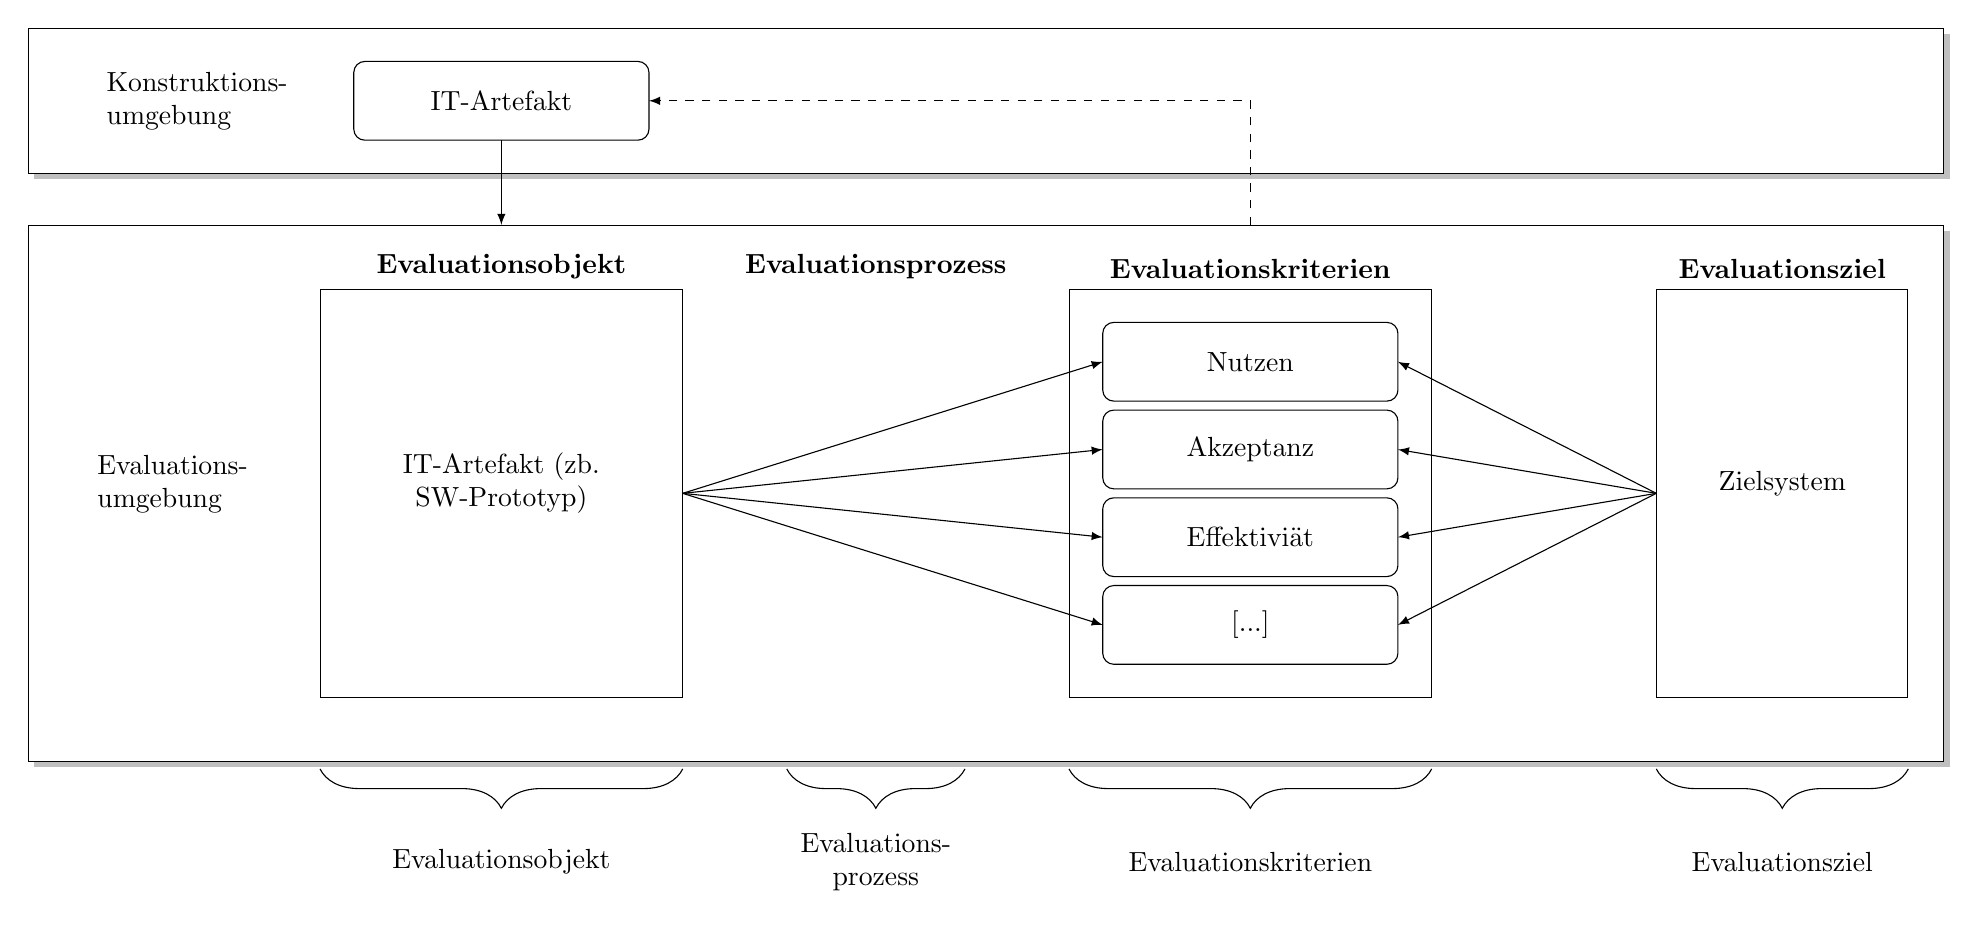
\begin{tikzpicture}
[auto,
decision/.style={diamond, draw=blue, thick, fill=blue!20,text width=4.5em,align=flush center,inner sep=1pt},
block/.style ={ rectangle, draw, fill=white,  text centered, minimum height=15mm, text width=12em},
block_todo/.style ={ rectangle, draw, fill=white,  text centered, minimum height=15mm, text width=12em, rounded corners, outer sep=5},
block_done/.style ={ rectangle, draw, fill=white,  text centered, minimum height=15mm, text width=12em, rounded corners, outer sep=5},
block_normal/.style ={ rectangle, draw, fill=white,  align= center, minimum height=1cm, text width=10em, rounded corners, outer sep=0},
block_exp/.style ={ rectangle, draw=none, fill=none,  text centered, minimum height=1.5cm, text width=12em,font=\bfseries, rounded corners, outer sep=0},
block_phantom/.style ={ block_normal, draw=none, fill=none},
block_background/.style ={ rectangle,  draw=black, fill=none,  text centered, minimum height=15mm,fill opacity=1, rounded corners=0, inner sep=25},
block_background_inner/.style ={ rectangle,  draw=black, fill=none,  text centered, minimum height=15mm,fill opacity=1, rounded corners=0, inner sep=12},
output/.style ={trapezium,draw,fill=none, minimum height=10mm,  align=center, trapezium left angle=60, trapezium right angle=120, text width=50},
line_inner/.style ={draw, -latex,shorten >=0pt, shorten <=0pt},
kreis/.style ={ circle, draw, fill=white,  text centered, minimum height=15mm, text width=10em, rounded corners, outer sep=0, minimum size=.4cm},
zylinder/.style={cylinder, draw, fill=yellow!20,shape border rotate=90, text height=5, align=center, aspect=.1, text width=10em, minimum height=6.5em, minimum width=2em},
line_outer/.style ={draw, -latex,shorten >=23pt, shorten <=0pt}]
]


\matrix (table) [column sep=1.5cm,row sep=1cm, ampersand replacement=\&,  nodes in empty cells, in front of path]
{
% row 1
\node [block_normal, draw=none, align=left, text width=10em] (11) {Konstruktions-umgebung};  \& [-2cm]
\node [block_normal] (12) {IT-Artefakt}; \& [-.5cm]
\node [block_phantom] (13) {};\& [-.5cm]
\node [block_phantom] (14) {};\& [1.5cm]
\node [block_phantom, text width=6em] (15) {};\\ [1.3cm]
 % row 2
\node [block_phantom, text width=10em] (21) {};\& 
\node [block_phantom] (22) {}; \&
\node [block_phantom] (23) {};\&
\node [block_normal] (24) {Nutzen};\&
\node [block_phantom, text width=6em] (25) {}; \\[-0.9cm]
 % row 3
\node [block_phantom, text width=10em] (31) {};\& 
\node [block_phantom] (32) {}; \&
\node [block_phantom] (33) {};\&
\node [block_normal] (34) {Akzeptanz};\&
\node [block_phantom, text width=6em] (35) {};   \\ [-0.9cm]
 % row 4
\node [block_phantom, text width=10em] (41) {};\& 
\node [block_phantom] (42) {}; \&
\node [block_phantom] (43) {};\&
\node [block_normal] (44) {Effektivi\"at};\&
\node [block_phantom, text width=6em] (45) {};    \\[-0.9cm]
 % row 5
\node [block_phantom, text width=10em] (51) {};\& 
\node [block_phantom] (52) {}; \&
\node [block_phantom] (53) {};\&
\node [block_normal] (54) {[...]};\&
\node [block_phantom, text width=6em] (55) {}; \\ [1cm]
  % row 6
 \node [block_phantom] (61) {};\& 
 \node [block_normal, rounded corners=0, draw=none] (62) {Evaluationsobjekt}; \&
 \node [block_normal, rounded corners=0, draw=none] (63) {Evaluations-\\prozess};\&
 \node [block_normal, rounded corners=0, draw=none] (64) {Evaluationskriterien};\&
 \node [block_normal, rounded corners=0, draw=none] (65) {Evaluationsziel}; \\[1cm]
};

\node[fit=(21)(51), block_background_inner, draw=none, align=left, inner xsep]{Evaluations-\\umgebung};
\node[fit=(22)(52), block_background_inner, label=\textbf{Evaluationsobjekt}](artefakt){IT-Artefakt (zb. SW-Prototyp)};
\node[fit=(23)(53), block_background_inner, text width=4em, draw=none,label=\textbf{Evaluationsprozess}](evaluation){};
\node[fit=(24)(54), block_background_inner, label=\textbf{Evaluationskriterien}](mess){};
\node[fit=(25)(55), block_background_inner, label=\textbf{Evaluationsziel}](ziel){Zielsystem};


\begin{scope}[on background layer]
\node[fit=(11)(15), block_background, drop shadow, fill=white, inner ysep=12]{};
\node[fit=(21)(55), block_background, drop shadow, fill=white,  inner ysep=35]{};
\end{scope}

%%Pfeile%%%
\draw [line_inner](ziel.west) to (24.east);
\draw [line_inner](ziel.west) to (34.east);
\draw [line_inner](ziel.west) to (44.east);
\draw [line_inner](ziel.west) to (54.east);
\draw[line_inner] (artefakt.east) to (24.west);
\draw[line_inner] (artefakt.east) to (34.west);
\draw [line_inner](artefakt.east) to (44.west);
\draw [line_inner](artefakt.east) to (54.west);
\draw [line_outer](12) to (artefakt);
\draw [line_outer,shorten <=23pt, shorten >=0pt, dashed](mess.north) |- (12.east);
 \draw [decorate, decoration={brace, amplitude=.5cm, raise=.9cm}](artefakt.south east) to (artefakt.south west);
 \draw [decorate, decoration={brace, amplitude=.5cm, raise=.9cm}](evaluation.south east) to (evaluation.south west);
 \draw [decorate, decoration={brace, amplitude=.5cm, raise=.9cm}](mess.south east) to (mess.south west);
 \draw [decorate, decoration={brace, amplitude=.5cm, raise=.9cm}](ziel.south east) to (ziel.south west);

%%%Background%%%%
% \begin{scope}[on background layer]
% \node[fit=(41)(63), block_background]{};
% \end{scope}
%%%Background%%%%


\end{tikzpicture}%
}%
{%file exists=false: befinde mich im root_verzeichnis
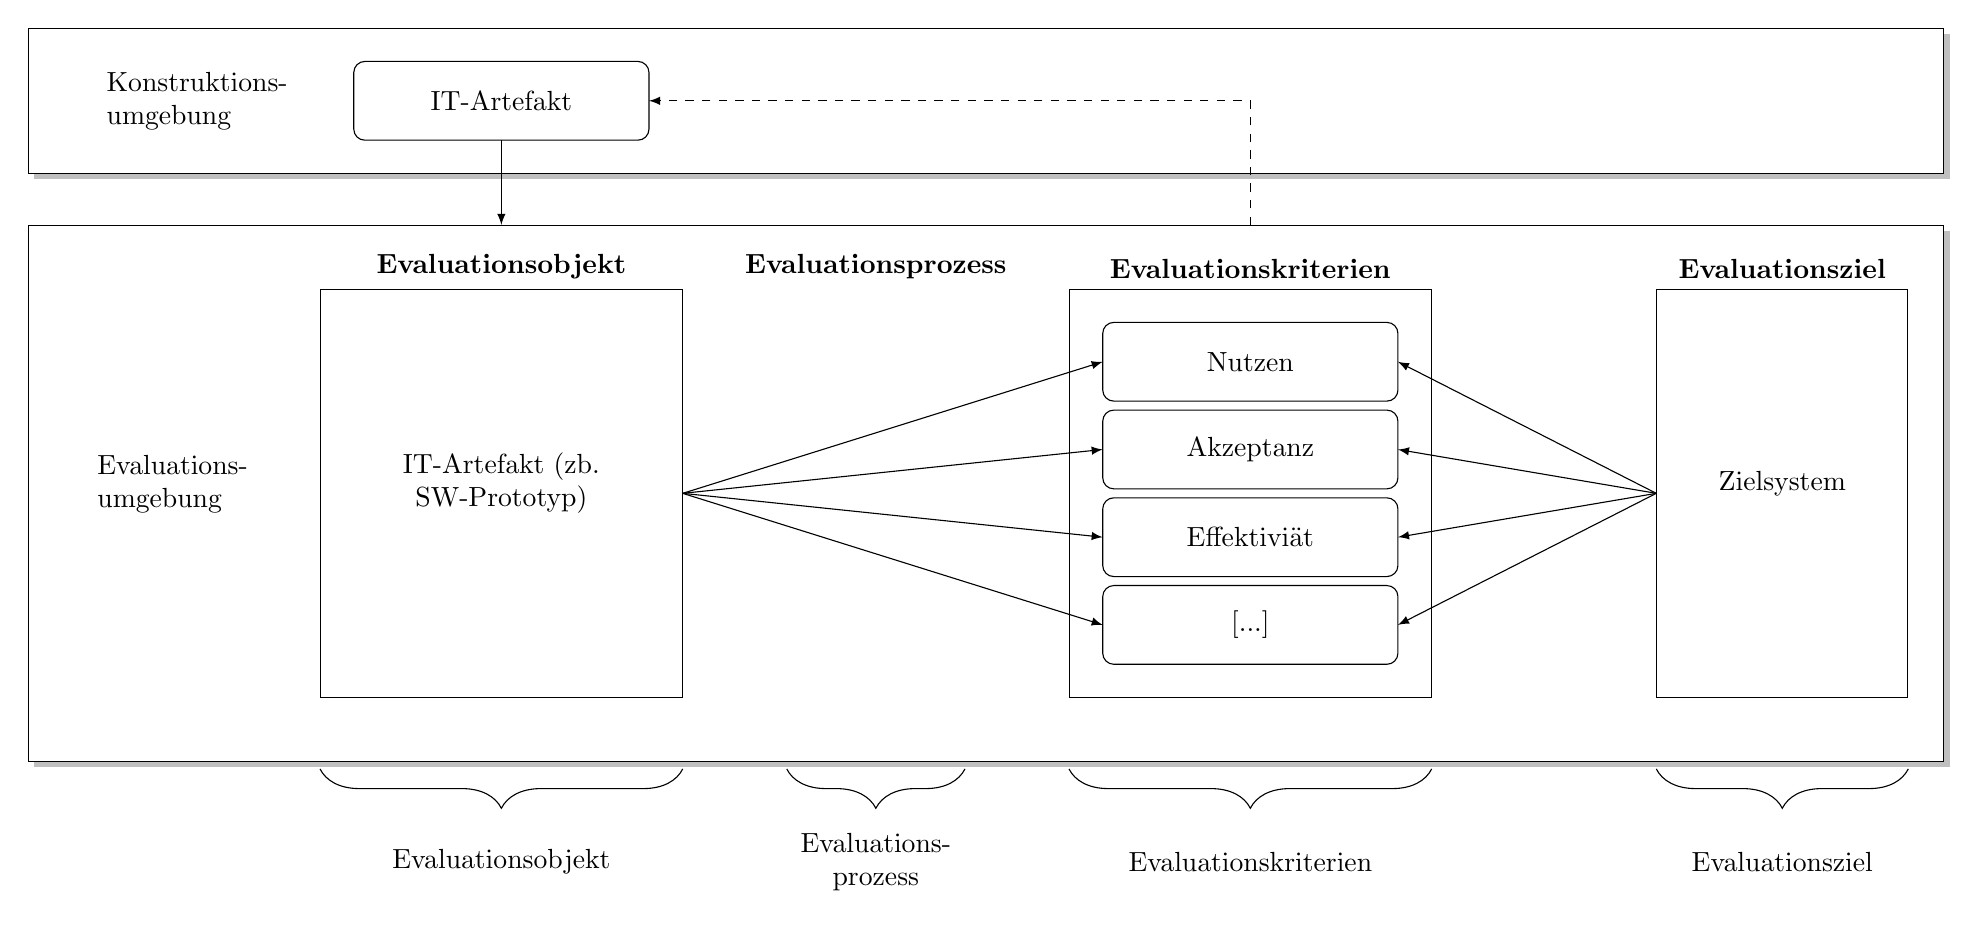
\begin{tikzpicture}
[auto,
decision/.style={diamond, draw=blue, thick, fill=blue!20,text width=4.5em,align=flush center,inner sep=1pt},
block/.style ={ rectangle, draw, fill=white,  text centered, minimum height=15mm, text width=12em},
block_todo/.style ={ rectangle, draw, fill=white,  text centered, minimum height=15mm, text width=12em, rounded corners, outer sep=5},
block_done/.style ={ rectangle, draw, fill=white,  text centered, minimum height=15mm, text width=12em, rounded corners, outer sep=5},
block_normal/.style ={ rectangle, draw, fill=white,  align= center, minimum height=1cm, text width=10em, rounded corners, outer sep=0},
block_exp/.style ={ rectangle, draw=none, fill=none,  text centered, minimum height=1.5cm, text width=12em,font=\bfseries, rounded corners, outer sep=0},
block_phantom/.style ={ block_normal, draw=none, fill=none},
block_background/.style ={ rectangle,  draw=black, fill=none,  text centered, minimum height=15mm,fill opacity=1, rounded corners=0, inner sep=25},
block_background_inner/.style ={ rectangle,  draw=black, fill=none,  text centered, minimum height=15mm,fill opacity=1, rounded corners=0, inner sep=12},
output/.style ={trapezium,draw,fill=none, minimum height=10mm,  align=center, trapezium left angle=60, trapezium right angle=120, text width=50},
line_inner/.style ={draw, -latex,shorten >=0pt, shorten <=0pt},
kreis/.style ={ circle, draw, fill=white,  text centered, minimum height=15mm, text width=10em, rounded corners, outer sep=0, minimum size=.4cm},
zylinder/.style={cylinder, draw, fill=yellow!20,shape border rotate=90, text height=5, align=center, aspect=.1, text width=10em, minimum height=6.5em, minimum width=2em},
line_outer/.style ={draw, -latex,shorten >=23pt, shorten <=0pt}]
]


\matrix (table) [column sep=1.5cm,row sep=1cm, ampersand replacement=\&,  nodes in empty cells, in front of path]
{
% row 1
\node [block_normal, draw=none, align=left, text width=10em] (11) {Konstruktions-umgebung};  \& [-2cm]
\node [block_normal] (12) {IT-Artefakt}; \& [-.5cm]
\node [block_phantom] (13) {};\& [-.5cm]
\node [block_phantom] (14) {};\& [1.5cm]
\node [block_phantom, text width=6em] (15) {};\\ [1.3cm]
 % row 2
\node [block_phantom, text width=10em] (21) {};\& 
\node [block_phantom] (22) {}; \&
\node [block_phantom] (23) {};\&
\node [block_normal] (24) {Nutzen};\&
\node [block_phantom, text width=6em] (25) {}; \\[-0.9cm]
 % row 3
\node [block_phantom, text width=10em] (31) {};\& 
\node [block_phantom] (32) {}; \&
\node [block_phantom] (33) {};\&
\node [block_normal] (34) {Akzeptanz};\&
\node [block_phantom, text width=6em] (35) {};   \\ [-0.9cm]
 % row 4
\node [block_phantom, text width=10em] (41) {};\& 
\node [block_phantom] (42) {}; \&
\node [block_phantom] (43) {};\&
\node [block_normal] (44) {Effektivi\"at};\&
\node [block_phantom, text width=6em] (45) {};    \\[-0.9cm]
 % row 5
\node [block_phantom, text width=10em] (51) {};\& 
\node [block_phantom] (52) {}; \&
\node [block_phantom] (53) {};\&
\node [block_normal] (54) {[...]};\&
\node [block_phantom, text width=6em] (55) {}; \\ [1cm]
  % row 6
 \node [block_phantom] (61) {};\& 
 \node [block_normal, rounded corners=0, draw=none] (62) {Evaluationsobjekt}; \&
 \node [block_normal, rounded corners=0, draw=none] (63) {Evaluations-\\prozess};\&
 \node [block_normal, rounded corners=0, draw=none] (64) {Evaluationskriterien};\&
 \node [block_normal, rounded corners=0, draw=none] (65) {Evaluationsziel}; \\[1cm]
};

\node[fit=(21)(51), block_background_inner, draw=none, align=left, inner xsep]{Evaluations-\\umgebung};
\node[fit=(22)(52), block_background_inner, label=\textbf{Evaluationsobjekt}](artefakt){IT-Artefakt (zb. SW-Prototyp)};
\node[fit=(23)(53), block_background_inner, text width=4em, draw=none,label=\textbf{Evaluationsprozess}](evaluation){};
\node[fit=(24)(54), block_background_inner, label=\textbf{Evaluationskriterien}](mess){};
\node[fit=(25)(55), block_background_inner, label=\textbf{Evaluationsziel}](ziel){Zielsystem};


\begin{scope}[on background layer]
\node[fit=(11)(15), block_background, drop shadow, fill=white, inner ysep=12]{};
\node[fit=(21)(55), block_background, drop shadow, fill=white,  inner ysep=35]{};
\end{scope}

%%Pfeile%%%
\draw [line_inner](ziel.west) to (24.east);
\draw [line_inner](ziel.west) to (34.east);
\draw [line_inner](ziel.west) to (44.east);
\draw [line_inner](ziel.west) to (54.east);
\draw[line_inner] (artefakt.east) to (24.west);
\draw[line_inner] (artefakt.east) to (34.west);
\draw [line_inner](artefakt.east) to (44.west);
\draw [line_inner](artefakt.east) to (54.west);
\draw [line_outer](12) to (artefakt);
\draw [line_outer,shorten <=23pt, shorten >=0pt, dashed](mess.north) |- (12.east);
 \draw [decorate, decoration={brace, amplitude=.5cm, raise=.9cm}](artefakt.south east) to (artefakt.south west);
 \draw [decorate, decoration={brace, amplitude=.5cm, raise=.9cm}](evaluation.south east) to (evaluation.south west);
 \draw [decorate, decoration={brace, amplitude=.5cm, raise=.9cm}](mess.south east) to (mess.south west);
 \draw [decorate, decoration={brace, amplitude=.5cm, raise=.9cm}](ziel.south east) to (ziel.south west);

%%%Background%%%%
% \begin{scope}[on background layer]
% \node[fit=(41)(63), block_background]{};
% \end{scope}
%%%Background%%%%


\end{tikzpicture}%
}%
\end{document}%